\section{Introduction to VGA}\label{sec:intro}
VGA (Video Graphics Array) is a visual graphics standard introduced in 1987.
It was developed to work with CRT (Cathode-Ray Tube) technology, which works 
by drawing each pixel in horizontal lines vertically down the display to 
create a \emph{frame}.

In order to produce the effect of a static image 
given only a single pixel controlled per instant, the entire frame 
would be redrawn (or `refreshed') quicker than the eye can perceive.
A refresh rate of \qty{60}{\Hz} would be typical.

Due to the physical deflection of an electron beam to produce pixels, 
extra time for the beam to adjust to a new line is included in the standard, called 
the \emph{blanking interval}. 
The start of a new line is controlled by the horizontal sync (hsync) signal, with a 
new frame in turn controlled by a vertical sync (vsync) signal. The blanking intervals before 
and after these signals are respectively called the \emph{front porch} and \emph{back porch}. 
In modern standards like HDMI, this extra time has been retained and instead carries extra 
data like accompanying audio. 


\subsection{Driving the display}\label{sec:drivingdisplay}

There are four requirements for driving a VGA display:
\begin{enumerate}
    \item Clock signal driving the display signal counters.
    \item Horizontal and vertical signals, defining pixels.
    \item Drawing graphical elements to the screen.
    \item Physical video output to a display.
\end{enumerate}

\subsubsection{Clock}
The required display frequency clock can be calculated by:
\begin{align*}
    f_{\text{clock}} & = L_h \times L_v \times f_{r}
\end{align*}

\begin{conditions}
    L_h & = & horizontal lines, 1903 \\
    L_v & = & vertical lines, 931 \\
    f_{r} & = & refresh frequency, \qty{60}{\Hz} \\
\end{conditions}

% where: 
% \begin{tabular}[H]{ l c l}
%     $\lambda$ & $=$ & wavelength \\
%     $v$ & $=$ & velocity, which in this case will be $c$, the speed of light \\
%     $f$ & $=$ & frequency \\
% \end{tabular}\\

The results in a required clock frequency of \qty{106.30158}{\MHz}. 
The easiest method of producing clock signals in Verilog is to divide down the main 
processor clock to the required subdivision. In the case of the 
Nexys A7, the onboard clock is \qty{100}{\MHz} and thus cannot be divided down to 
a value that is greater. However, by using the Clocking Wizard IP provided by Xilinx, 
this can be produced. The caveat is that it will not be necessarily exact. 
In this case, the actual output clock is \qty{106.296}{\MHz}, which is within \qty{0.005}{\percent}.

\subsubsection{Signals}
In this implementation, the horizontal and vertical signals are controlled by counters 
operating at the overall display frequency, determining which pixel is being drawn. 
The counter values then determine the widths of each signal parameter.
The parameters are outlined in \cref{table:vgaparams}, which informs the display dimensions
as shown in \cref{fig:vga}.
\begin{xltabular}{\linewidth}{Y|YYYY}
    & Sync signal & Back porch & Display & Front porch \\
    \hline
    Horizontal & 151 & 384 & 1824 & 1903 \\
    \hline
    Vertical & 2 & 30 & 930 & 931 \\
    \hline
    \caption{VGA signal parameters}\label{table:vgaparams}
\end{xltabular}
The visible portion produces a display resolution of 1440x900. 

\begin{figure}[htbp]
    \centering
    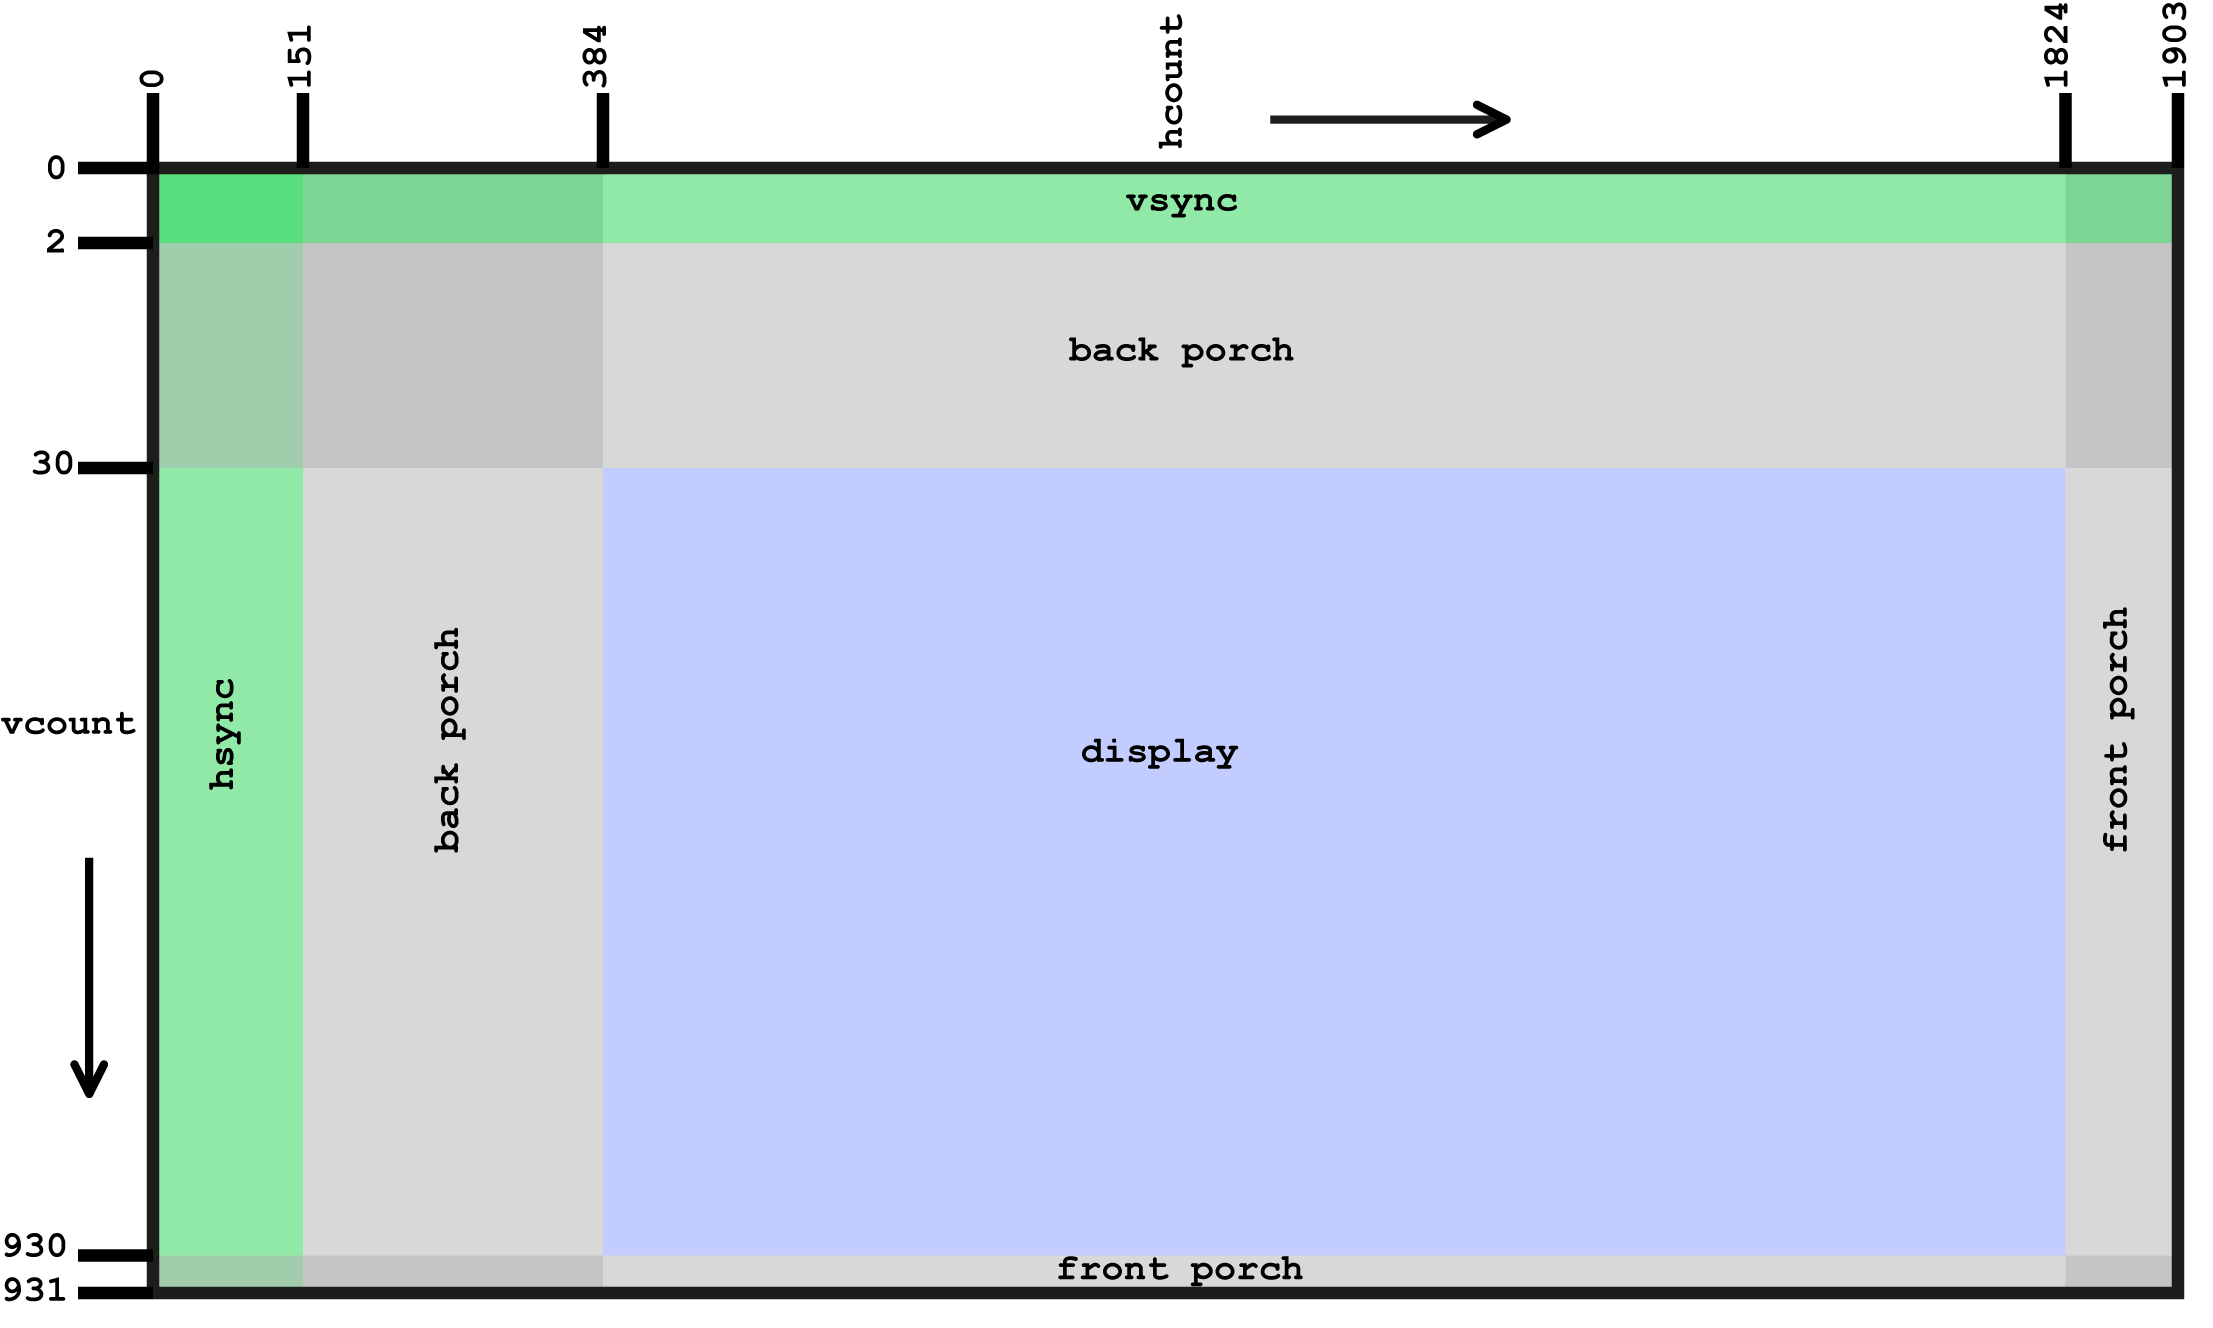
\includegraphics[width=0.8\textwidth]{./figures/vga display.png}
    \caption{Display parameters}\label{fig:vga}
\end{figure}

\subsubsection{Drawing graphics}
Graphics drawing is delegated to its own module\footnote{
    \Cref{sec:drawcon}.
} separate from the VGA controller. 
To provide an overview, the graphics drawing module (draw controller) takes as input the 
current pixel by coordinates in \emph{x} and \emph{y} with reference to the top left corner
of the visible display. It outputs the colour for this pixel as a 12-bit hexadecimal number, which can then 
be passed to the VGA port.

\subsubsection{Video output}
The specifics of the output (i.e. required voltages, pin connections etc. to the D-sub connector) is
abstracted away in the constraints file for the board. In this file, the pins of the Nexys A7 
with regard to the VGA port are provided and simply need to be 
included in the compilation to be used. 

The colour channels in the port are different physical connections, taking up six pins of the 
connector - one each for red, green, and blue, in addition to each colour's ground reference. 
In the implementation for this project, the 4-bit output colour variables
(\lstinline{VGA_R}, \lstinline{VGA_G}, \lstinline{VGA_B}) 
have been merged into a single 12-bit variable (\lstinline{colour}). 

The mapping occurs as follows:

\begin{tabular}{l|lll}
    Original & \lstinline|VGA_R[3:0]| & \lstinline|VGA_G[3:0]| & \lstinline|VGA_B[3:0]| \\
    Implementation & \lstinline|colour[11:8]| & \lstinline|colour[7:4]| & \lstinline|colour[3:0]| 
\end{tabular}
% \begin{lstlisting}[numbers=none,frame=none]
%         Original        |    VGA_R[3:0]     VGA_G[3:0]      VGA_B[3:0]
%         Implementation  |    colour[11:8]   colour[7:4]     colour[3:0] 
% \end{lstlisting}

The advantage of this is that colour assignment to a pixel can now be encoded as a single hexadecimal number 
with three digits - the first encoding the red value, the second green, and the third blue. 
This is particularly useful as the encoding now follows web-safe hexadecimal colour space\footnote{
    A palette reference available at \href{https://www.rapidtables.com/web/color/Web_Safe.html}{RapidTables \faExternalLink}.
}, reducing the guesswork in developing a colour on screen.

\subsection{Limitations}
With VGA as the only display adapter available on the board, the colours available is limited 
to 4-bits for the red, green, and blue channels each. This results in 4096 total colours. 
Most modern monitor displays, on the other hand, permit over 16 million colours due to the 
use of 24-bit colour space. 

\subsection{Implementation}
The implementation of the VGA controller can be found in \cref{code:vga}.